\section{{\system}使用例}

% 本章では{\system}を利用した様々な入力/編集作業の例を示す。

\subsection{日本語入力}

{\system}は、
MacRuby\footnote{
  RubyをMac用に拡張したもので、あらゆるMacのAPIをRubyから利用することができる。
}で記述された日本語IMEである「Gyaim\footnote{
 \textsf{https://github.com/masui/Gyaim}
}」に様々な編集機能を追加したものである。
%
図\ref{japaneseinput}は{\system}による日本語入力の例である。
IMEはアルファベット以外の文字を入力するときだけ有効にするのが普通であるが、
{\system}は、編集操作を行うために常に有効であることを想定して実装した。
そのため、英語入力と日本語入力の両方が可能である。

\begin{figure}[H]
\centerline{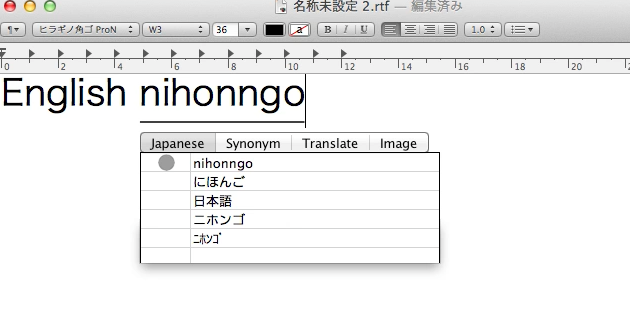
\includegraphics[width=70mm,bb=0 0 600 320]{figures/japanese.png}}
\caption{{\system}による日本語入力の例.}
\label{japaneseinput}
\end{figure}

\subsection{ブロック移動}

テキストの一部を別の場所に移動する操作は
テキストエディタの重要な機能のひとつであるが、
エディタによって操作方法が大きく異なっている。
たとえばEmacsでテキストを移動させたい場合は、
移動する領域をキー操作によって指定してから削除/コピーし、
カーソルを移動してからペーストするという手順を利用するのに対し、
ブラウザの編集領域でテキストを移動させたい場合は、
マウスで領域を指定した後で選択領域をドラッグして別の位置に移動することが多い。
このように、テキスト移動のような基本操作でもエディタごとに操作が異なっているのは不便であり、
操作ミスをしがちであるが、
{\system}を利用するとあらゆるエディタにおいて
同じ操作でテキストを移動することができる。

図\ref{move1}はMac OSに標準登載されている
「テキストエディット」でテキストを編集しているところである。

\begin{figure}[H]
\centerline{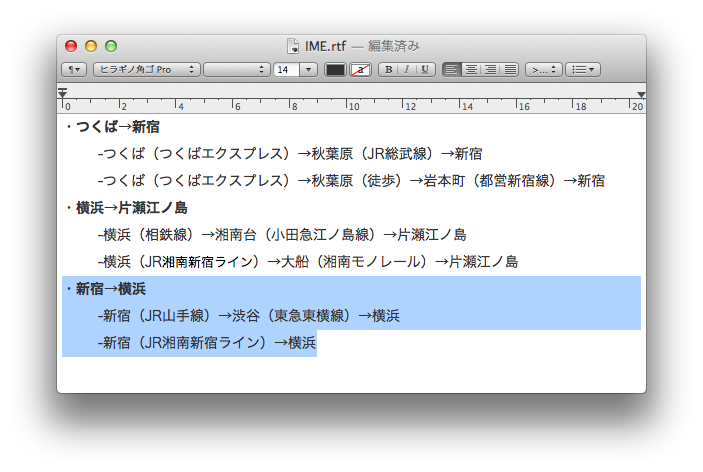
\includegraphics[width=70mm,bb=0 0 703 472]{figures/block2.png}}
\caption{ブロック移動前の状態.}
\label{move1}
\end{figure}

ここでShift+↑キーを押すとテキストは図\ref{move2}のように変化する。

\begin{figure}[H]
\centerline{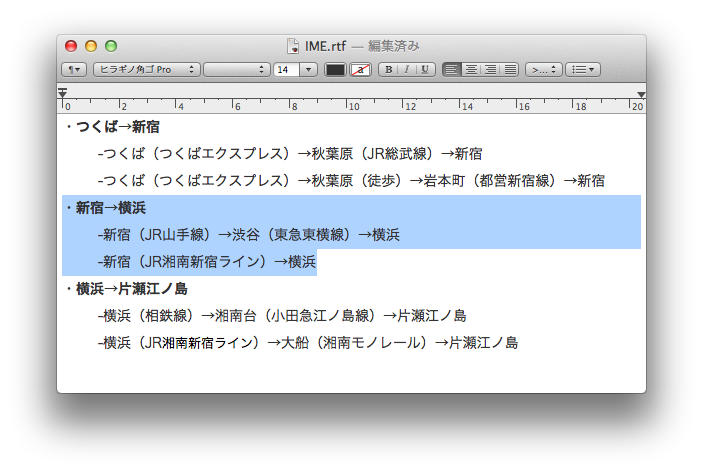
\includegraphics[width=70mm,bb=0 0 703 472]{figures/block3.png}}
\caption{Shift+↑キーを押した後の状態.}
\label{move2}
\end{figure}

図\ref{move3}はブラウザ上でGoogle Docsのテキストを編集しているところである。
ここでShift+↓キーを二度押すと、テキストは図\ref{move4}のように変化する。

\begin{figure}[H]
\centerline{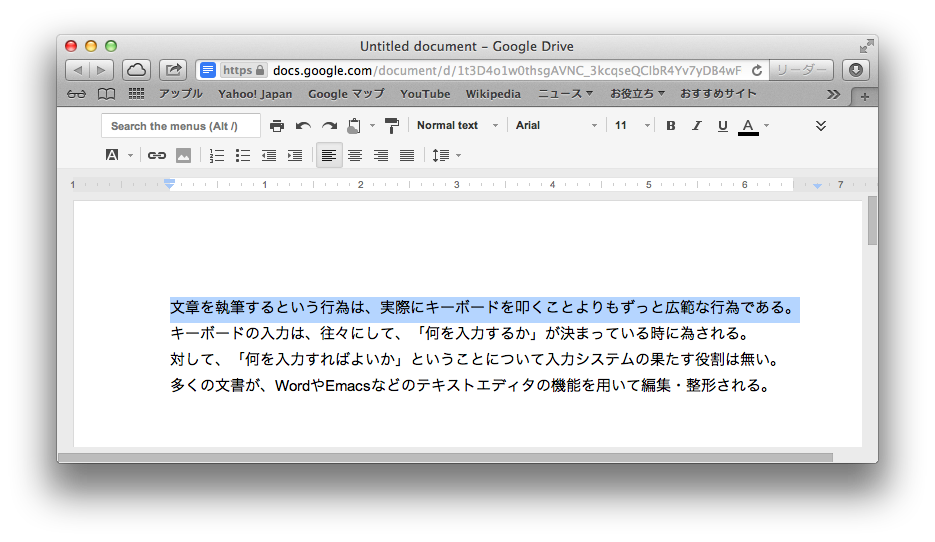
\includegraphics[width=70mm,bb=0 0 935 542]{figures/block4.png}}
\caption{ブロック移動前の状態.}
\label{move3}
\end{figure}

\begin{figure}[H]
\centerline{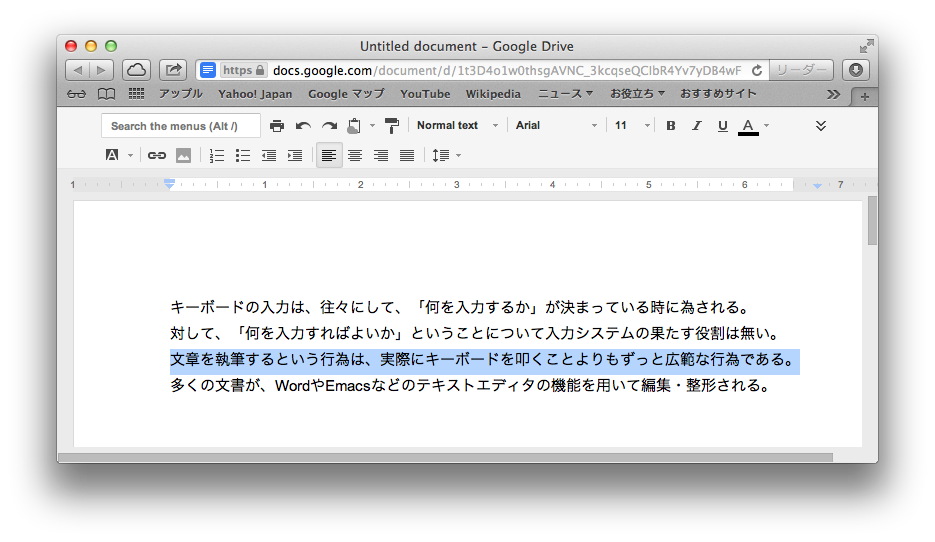
\includegraphics[width=70mm,bb=0 0 935 542]{figures/block5.png}}
\caption{キーを押した後の状態.}
\label{move4}
\end{figure}

このように、あらゆるエディタにおいて
Shift+矢印キーという共通の操作で
ブロック移動を行なうことができることがわかる。

\subsection{連続インデント}

前述したブロック移動は、インデントを調整する機能も備えている。
プログラミングを行なっている時だけでなく、
普通のテキストを編集している場合でも
行頭の空白やタブの量を調整するインデント処理は頻繁に行われるが、
自動的にインデントを行うエディタもあれば、
コマンドを打ち込まなければならないものもあり、
そのような調整機能を持っていないエディタも多い。
{\system}を利用すると、あらゆるエディタや入力フィールドでブロック移動と同時にインデントが自動で行われる。

図\ref{indent1}は、Xcode上でPythonプログラムを書いている例である。
Xcodeは、Objective-CやRubyなどの言語で自動インデントの機能を備えているが、Pythonには対応していない。
たとえば、図\ref{indent1}のようなテキストに対して
図\ref{indent2}のように移動させたいブロックを選択し、Shift+↓キーを入力することで、テキストは図\ref{indent3}のように変化する。

\begin{figure}[H]
\centerline{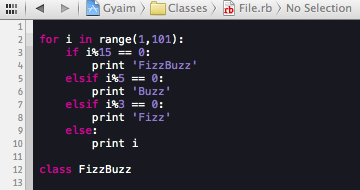
\includegraphics[width=70mm,bb=0 0 360 190]{figures/indent1.png}}
\caption{ブロック移動前の状態}
\label{indent1}
\end{figure}

\begin{figure}[H]
\centerline{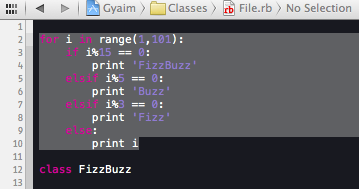
\includegraphics[width=70mm,bb=0 0 360 190]{figures/indent2.png}}
\caption{テキストを選択した状態}
\label{indent2}
\end{figure}

\begin{figure}[H]
\centerline{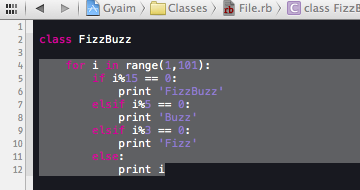
\includegraphics[width=70mm,bb=0 0 360 190]{figures/indent3.png}}
\caption{ブロック移動後の状態}
\label{indent3}
\end{figure}

このように、あらゆるエディタにおいて、ブロック移動を行う際に適切な空白とタブを自動で補完することができる。

\subsection{単語置換}

多くのエディタが単語の検索/置換機能を持っているが、
その操作方法はシステムごとに異なっている。
例えば、コンソール上で検索と置換を行う時はgrepやsedコマンドを用いるが、多くのエディタソフトではControl+FやCommand+Fが用意されている。

{\system}を利用することでこの操作を共通化する例を挙げる。

あらかじめめ割り当てたファンクションキーを押すと、
図\ref{search1}のように{\system}の単語置換ウィンドウが起動する。

\begin{figure}[H]
\centerline{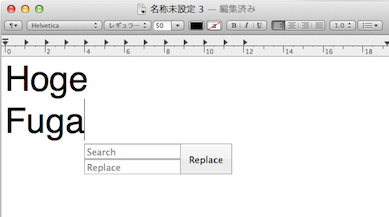
\includegraphics[width=70mm,bb=0 0 360 215]{figures/replace1.png}}
\caption{単語置換ウィンドウの例}
\label{search1}
\end{figure}

図\ref{search2}のように、入力語と置換語をテキストエリアに打ち込み、Replaceボタンを押すと、

\begin{figure}[H]
\centerline{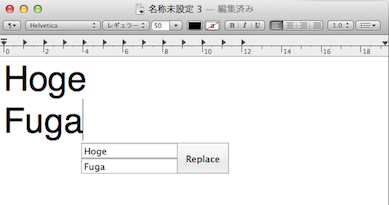
\includegraphics[width=70mm,bb=0 0 360 191]{figures/replace2.png}}
\caption{置換ウィンドウに単語を入力した例}
\label{search2}
\end{figure}


テキストは図\ref{search3}のように置換される。

\begin{figure}[H]
\centerline{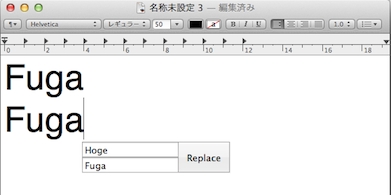
\includegraphics[width=70mm,bb=0 0 360 191]{figures/replace3.png}}
\caption{単語置換後の状態}
\label{search3}
\end{figure}

このように、あらゆるエディタ上で検索と置換が可能である。

\subsection{Dynamic Macro}

Emacsではlispプログラムでエディタの機能を拡張することが出来るが、
これらのスクリプトをIME上に実装することで、
他のエディタ上でもEmacsと同様の拡張機能を動作させることができる。

以下に{\system}でDynamic Macro\cite{DynamicMacro}を実現した例を挙げる。
Dynamic Macroは、入力の繰り返しを自動化するEmacs拡張であるが、
{\system}ではこれと同様の機能をRubyで実装している。
図\ref{dynamic1}のように、ユーザの入力操作が繰り返しになっているとき、
任意に設定したファンクションキーを押すと、テキストは図\ref{dynamic2}のように編集される。

\begin{figure}[H]
\centerline{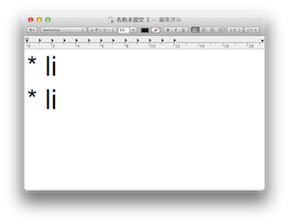
\includegraphics[width=80mm,bb=0 0 360 220]{figures/dynamic1.png}}
\caption{Dynamic Macro機能を使用する前のテキスト}
\label{dynamic1}
\end{figure}

\begin{figure}[H]
\centerline{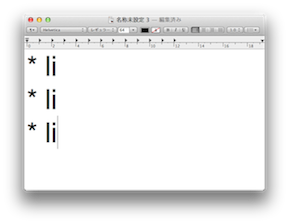
\includegraphics[width=80mm,bb=0 0 360 220]{figures/dynamic2.png}}
\caption{Dynamic Macro機能を使用した後のテキスト}
\label{dynamic2}
\end{figure}


以下は{\system}のDynamic Macro機能をブラウザのアドレスバー上で実行した例である。
図\ref{dynamic3}のように、ユーザの入力に"abc"が繰り返されているとき、
任意に設定したファンクションキーを押すと、テキストは図\ref{dynamic4}のように編集される。

\begin{figure}[H]
\centerline{
\includegraphics[width=70mm,bb=0 0 360 50]{figures/dynamic3.png}}
\caption{Dynamic Macro機能を使用する前のテキスト}
\label{dynamic3}
\end{figure}

\begin{figure}[H]
\centerline{
\includegraphics[width=70mm,bb=0 0 360 50]{figures/dynamic4.png}}
\caption{Dynamic Macro機能を使用した後のテキスト}
\label{dynamic4}
\end{figure}

Emacs上に実装されたDynamic MacroはEmacs上でしか利用できないが、
{\system}上に実装されたDynamic Macroは
あらゆるテキストエディタの上で利用することができる。


